\section{Introduction}
\label{sec:intro}

% Para 1: Background - financial MAS landscape
Large language models have enabled a new generation of financial multi-agent systems that decompose complex trading decisions across specialized roles. TradingAgents~\cite{tradingagents2025} coordinates fundamental, sentiment, and technical analysts through structured debate; FinCon~\cite{fincon2024} introduces a manager-analyst hierarchy with conceptual verbal reinforcement; R\&D-Agent~\cite{rdagent2025} automates quantitative factor research through a Research-Development-Feedback loop. These systems demonstrate that multi-agent collaboration outperforms monolithic approaches on standard backtesting benchmarks.
% 中文：大语言模型催生了新一代金融多智能体系统，将复杂交易决策分解到专业化角色中。TradingAgents 通过结构化辩论协调基本面、情绪和技术分析师；FinCon 引入管理者-分析师层级与概念性语言强化；RD-Agent 通过研究-开发-反馈循环自动化量化因子研究。这些系统证明多智能体协作在标准回测基准上优于单体方法。

\begin{figure*}[t]
\centering
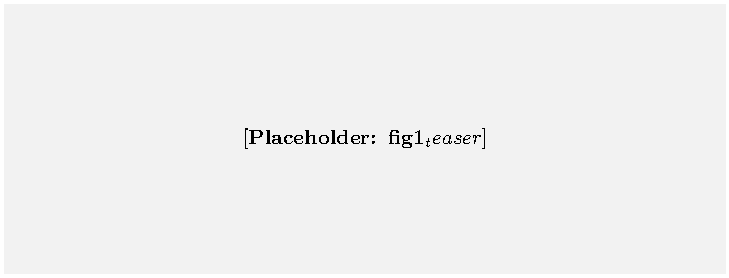
\includegraphics[width=\linewidth]{figures/fig1_teaser.pdf}
\caption{Comparison of self-improvement paradigms in financial multi-agent systems. Left: existing systems rely on verbal reinforcement (open loop). Center: empirical evidence of failure---frontier models lose money in live trading~\cite{deepfund2025} and RL finetuning causes reward hacking~\cite{losingwinner2025}. Right: \textsc{FinOPD} addresses these failures through three design insights: hindsight PnL as privileged information, Shapley-weighted credit assignment, and parametric-nonparametric complementarity.}
\label{fig:teaser}
\end{figure*}

% Para 2: The problem - verbal reinforcement is insufficient
However, the self-improvement mechanisms in these systems remain confined to the prompt level (Figure~\ref{fig:teaser}, left). Verbal reinforcement~\cite{reflexion2023} summarizes past trading reflections into natural-language beliefs prepended to future prompts, but risk-adjusted returns, drawdown statistics, and regime-dependent performance signals never reach model parameters or consolidate into retrievable memory. Recent evidence exposes the consequences of this limitation (Figure~\ref{fig:teaser}, center): a twelve-month live benchmark shows that even frontier closed-source models incur net losses in real trading~\cite{deepfund2025}, and reinforcement-finetuned LLM agents achieve higher directional accuracy yet lower cumulative returns~\cite{losingwinner2025}, a reward-hacking failure arising from optimizing prediction accuracy rather than portfolio-level profitability.
% 中文：然而，这些系统的自我改进机制仍局限于 prompt 层面。语言强化将过去的交易反思总结为自然语言信念并前置到未来 prompt 中，但风险调整收益、回撤统计和 regime 相关的表现信号从未到达模型参数或固化为可检索的记忆。最近的证据暴露了这一局限的后果：十二个月的实盘基准显示即使前沿闭源模型也在真实交易中净亏损，强化微调的 LLM agent 方向准确率更高但累计收益更低——这是优化预测准确率而非组合级盈利性导致的 reward hacking 失败。

% Para 3: Why existing solutions don't work
The broader LLM community has developed on-policy self-distillation~\cite{opsd2026,gkd2024} and trajectory-level self-evolution~\cite{seagent2025,seea2025} methods that update model parameters from experience. These approaches consistently outperform prompt-only alternatives in mathematical reasoning and code generation. However, direct application to financial multi-agent systems faces three obstacles absent in single-model settings: (i) the privileged information for the teacher is undefined, since ground-truth does not exist in finance and prediction accuracy leads to reward hacking; (ii) credit must be assigned across multiple specialist agents whose contributions to a trajectory are entangled; (iii) financial markets exhibit both slow distributional drift and recurring concrete patterns, requiring mechanisms beyond pure parametric adaptation.
% 中文：更广泛的 LLM 社区已开发了在线策略自蒸馏和轨迹级自进化方法，从经验中更新模型参数。这些方法在数学推理和代码生成中一致优于仅 prompt 的替代方案。然而，直接应用于金融多智能体系统面临单模型设置中不存在的三个障碍：(i) 教师的特权信息未定义，因为金融中不存在 ground-truth 且预测准确率导致 reward hacking；(ii) 必须在多个专家 agent 之间分配信用，它们对轨迹的贡献是纠缠的；(iii) 金融市场同时展现缓慢的分布漂移和反复出现的具体模式，需要超越纯参数适应的机制。

% Para 4: Our approach
We propose \textsc{FinOPD}, a financial multi-agent framework that addresses these obstacles through three design decisions. First, we condition the teacher on hindsight risk-adjusted PnL (Sharpe, MDD, CVaR) rather than directional labels, anchoring distillation directly to profitability. Second, we introduce Shapley-weighted distillation that estimates each agent's marginal contribution via subset replay and weights the learning signal accordingly. Third, we complement parametric evolution with a non-parametric belief store that indexes winning geometry-factor-action triples by visual-geometric embeddings, preserving concrete patterns that gradient averaging would dilute. Supporting these mechanisms, a Visual-Geometric Encoder provides structured chart primitives as a shared semantic layer, and a Geometry-Conditioned Factor Router models tool selection as a learnable discrete policy over a library of 160 pre-mined alpha factors.
% 中文：我们提出 FinOPD，一个通过三个设计决策解决上述障碍的金融多智能体框架。第一，我们将教师条件化于事后风险调整 PnL（Sharpe、MDD、CVaR）而非方向标签，将蒸馏直接锚定于盈利性。第二，我们引入 Shapley 加权蒸馏，通过子集重放估计每个 agent 的边际贡献并相应加权学习信号。第三，我们用非参数 belief 存储补充参数进化，通过视觉几何嵌入索引获胜的几何-因子-动作三元组，保留梯度平均会稀释的具体模式。作为支撑，视觉几何编码器提供结构化图表原语作为共享语义层，几何条件化因子路由器将工具选择建模为在 160 个预挖掘 alpha 因子库上的可学习离散策略。

% Para 5: Contributions
Our contributions are as follows:
\begin{itemize}[leftmargin=*,nosep]
\item We formulate the self-evolution problem for financial multi-agent systems and identify three design questions (privileged information, credit assignment, parametric sufficiency) that distinguish it from single-model self-distillation.
\item We propose \textsc{FinOPD}, integrating on-policy self-distillation with hindsight PnL conditioning, Shapley-weighted credit assignment, and a retrieval-augmented belief store into a unified dual-track evolution framework.
\item We conduct extensive experiments on Dow-30 and CSI-300 benchmarks with twelve baselines, ten ablations, and strict post-cutoff evaluation, demonstrating state-of-the-art performance in Sharpe ratio, drawdown control, and cross-regime robustness.
\end{itemize}
% 中文：我们的贡献如下：(1) 形式化金融多智能体系统的自进化问题，识别三个设计问题（特权信息、信用分配、参数充分性）使其区别于单模型自蒸馏；(2) 提出 FinOPD，将在线策略自蒸馏与事后 PnL 条件化、Shapley 加权信用分配和检索增强 belief 存储整合为统一的双轨进化框架；(3) 在 Dow-30 和 CSI-300 基准上进行广泛实验，包含十二个基线、十组消融和严格的 post-cutoff 评估，展示在夏普比率、回撤控制和跨 regime 鲁棒性上的 SOTA 表现。
